% Provenance (never printed): cycle 3 "Matiere, mouvement, energie,
% information" and "La planete Terre" (meteorological phenomena, the water in
% the air, measuring the weather); see sources/book1/PROVENANCE.md.
% Book 1, grade 4, chapter 1.
\chapter{Awan, Hujan, dan Salju}\label{ch:g4:clouds-rain-snow}

Siang itu panas, di musim panas. Waktu makan siang, langit biru, dengan
beberapa \omterm{def:g4:clouds-rain-snow:cloud}{awan} putih kecil seperti gumpalan kapas. Pada pukul tiga, salah
satu \omterm{def:g4:clouds-rain-snow:cloud}{awan} itu sudah tumbuh. \omterm{def:g4:clouds-rain-snow:cloud}{Awan} itu menggelembung ke atas, makin lama
makin tinggi, seperti kembang kol putih yang berdiri di atas alas kelabu
yang datar. Puncaknya melebar. Alasnya menjadi gelap. Angin sejuk bertiup
kencang, tetes-tetes besar yang pertama jatuh, dan selama dua puluh menit
\omterm{def:g4:clouds-rain-snow:precipitation}{hujan} turun dengan deras. Lalu \omterm{def:g4:clouds-rain-snow:cloud}{awan} itu bergeser pergi, matahari muncul
kembali, dan trotoar yang basah mengepulkan uap.

Dari mana datangnya \omterm{def:g4:clouds-rain-snow:cloud}{awan} itu? Terbuat dari apa \omterm{def:g4:clouds-rain-snow:cloud}{awan} itu? Dan berapa banyak
\omterm{def:g4:clouds-rain-snow:precipitation}{hujan} yang turun dalam dua puluh menit itu?

\begin{recall}
\omterm{def:g1:watching-the-weather:weather}{Cuaca} adalah keadaan udara di suatu tempat dan pada suatu waktu: cerah,
berawan, \omterm{def:g4:clouds-rain-snow:precipitation}{hujan}, bersalju, berangin, berkabut; kita mencatatnya pada \omterm{def:g1:watching-the-weather:weather-chart}{tabel
cuaca} (\cref{ch:g1:watching-the-weather}). Air dari \omterm{def:g2:water-on-earth:ocean}{laut}, \omterm{def:g1:landscapes-around-us:water}{danau}, dan tanah
naik ke udara, lalu turun kembali sebagai \omterm{def:g4:clouds-rain-snow:precipitation}{hujan}
(\cref{ch:g2:water-on-earth}). Buku fisika menceritakan bagaimana air
menguap (dari cair menjadi gas yang tidak terlihat), mengembun (dari gas
kembali menjadi tetes-tetes cairan yang sangat kecil), dan membeku (dari
cair menjadi es), serta bagaimana termometer mengukur suhu dalam derajat
Celsius.
\end{recall}

\section{Apa itu awan?}

Udara di sekitar kita selalu mengandung sedikit air, dalam bentuk gas yang
tidak terlihat: uap air. Ketika udara naik, udara itu mendingin. Ketika
sudah cukup dingin, sebagian uap airnya mengembun menjadi titik-titik air
yang begitu kecil sehingga embusan udara yang paling lemah pun membuatnya
tetap melayang. Miliaran titik air ini, berdampingan, membentuk \omterm{def:g4:clouds-rain-snow:cloud}{awan} yang
bisa kita lihat. Di tempat yang tinggi, tempat udara sangat dingin,
titik-titik air itu membeku, dan \omterm{def:g4:clouds-rain-snow:cloud}{awan} tersusun dari kepingan es yang
sangat kecil.

\begin{definition}[Awan dan kabut]\label{def:g4:clouds-rain-snow:cloud}
Yang disebut \emph{awan}\index{awan} adalah sejumlah besar titik air yang
sangat kecil, atau kepingan es yang sangat kecil, yang bersama-sama
melayang di udara. Yang disebut \emph{kabut}\index{kabut} adalah awan yang
menyentuh tanah.
\end{definition}

\begin{example}[Napasmu pada pagi yang dingin]\label{ex:g4:clouds-rain-snow:breath}
Pada pagi yang dingin, napasmu membentuk \omterm{def:g4:clouds-rain-snow:cloud}{awan} putih kecil di depan mulutmu.
Udara yang kamu embuskan hangat dan mengandung uap air. Udara yang dingin
segera mendinginkannya, uap itu mengembun menjadi titik-titik air yang
sangat kecil --- dan muncullah \omterm{def:g4:clouds-rain-snow:cloud}{awan} mini, yang lalu lenyap ketika
titik-titik airnya menguap lagi.
\end{example}

\omterm{def:g4:clouds-rain-snow:cloud}{Awan} berwarna putih karena titik-titik airnya menghamburkan sinar matahari
ke segala arah. Jika \omterm{def:g4:clouds-rain-snow:cloud}{awan} itu sangat tebal, hanya sedikit cahaya yang
sampai ke alasnya, dan dari bawah \omterm{def:g4:clouds-rain-snow:cloud}{awan} itu tampak kelabu, atau hampir
hitam: itulah tanda \omterm{def:g4:clouds-rain-snow:cloud}{awan} yang berat, penuh air.

\section{Golongan-golongan awan}

\omterm{def:g4:clouds-rain-snow:cloud}{Awan} mempunyai banyak bentuk, dan para pengamat \omterm{def:g1:watching-the-weather:weather}{cuaca} di seluruh dunia
memilahnya dengan cara yang sama, menurut bentuknya dan menurut ketinggian
tempatnya melayang.

\begin{definition}[Golongan awan]\label{def:g4:clouds-rain-snow:cloud-families}
Keempat golongan \omterm{def:g4:clouds-rain-snow:cloud}{awan} yang perlu diketahui adalah:
\begin{itemize}
  \item \emph{kumulus}\index{kumulus}: \omterm{def:g4:clouds-rain-snow:cloud}{awan} bertumpuk, putih dan
        menggelembung, dengan alas yang datar, seperti gumpalan kapas;
  \item \emph{stratus}\index{stratus}: \omterm{def:g4:clouds-rain-snow:cloud}{awan} berlapis, lembaran kelabu yang
        datar yang menutupi seluruh langit, di tempat yang rendah;
  \item \emph{sirus}\index{sirus}: \omterm{def:g4:clouds-rain-snow:cloud}{awan} berserat, berupa benang atau ikal
        putih yang tipis, sangat tinggi, tersusun dari es;
  \item \emph{kumulonimbus}\index{kumulonimbus}: \omterm{def:g4:clouds-rain-snow:cloud}{awan} badai, menara raksasa
        yang menjulang dari alas yang rendah dan gelap sampai ketinggian
        yang sangat besar, dan puncaknya sering melebar dan datar.
\end{itemize}
\end{definition}

Nama-nama itu berasal dari kata Latin: \emph{cumulus} berarti tumpukan,
\emph{\omterm{def:g4:clouds-rain-snow:cloud-families}{stratus}} lapisan, \emph{cirrus} ikal rambut, dan \emph{nimbus} \omterm{def:g4:clouds-rain-snow:cloud}{awan}
\omterm{def:g4:clouds-rain-snow:precipitation}{hujan}.

\begin{omfigure}
\begin{minipage}[b]{0.49\linewidth}\centering
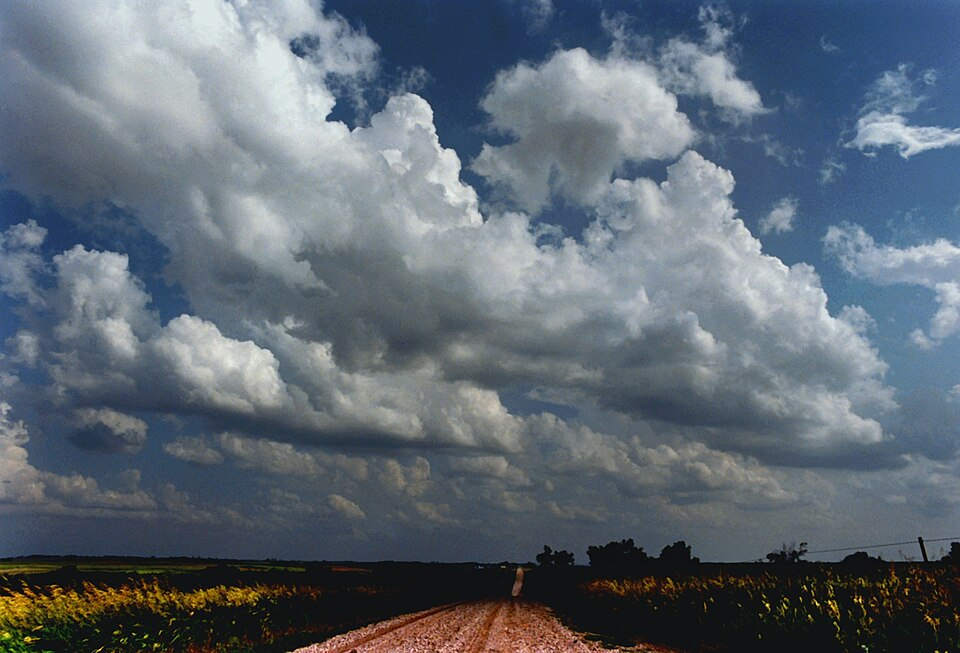
\includegraphics[width=\linewidth]{images/book1/g4-cumulus.jpg}

{\small \omterm{def:g4:clouds-rain-snow:cloud-families}{Kumulus}, \omterm{def:g4:clouds-rain-snow:cloud}{awan} bertumpuk dengan alas yang datar.}
\end{minipage}\hfill
\begin{minipage}[b]{0.49\linewidth}\centering
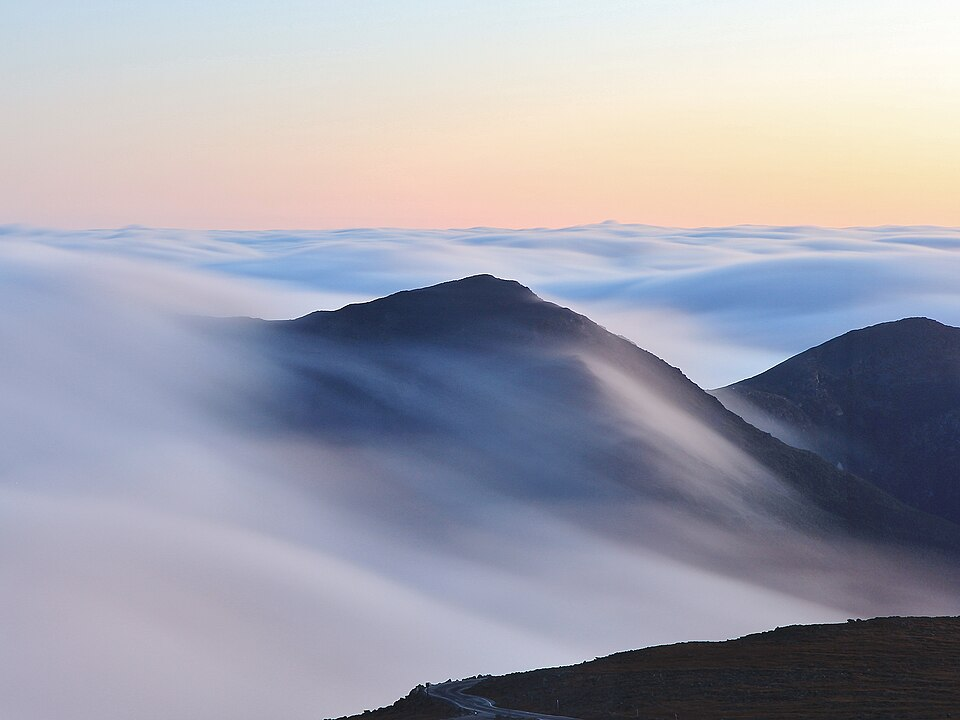
\includegraphics[width=\linewidth]{images/book1/g4-stratus.jpg}

{\small \omterm{def:g4:clouds-rain-snow:cloud-families}{Stratus}: lapisan yang datar, di sini dilihat dari atas, dari sebuah \omterm{def:g1:landscapes-around-us:landform}{gunung}.}
\end{minipage}

\medskip
\begin{minipage}[b]{0.49\linewidth}\centering
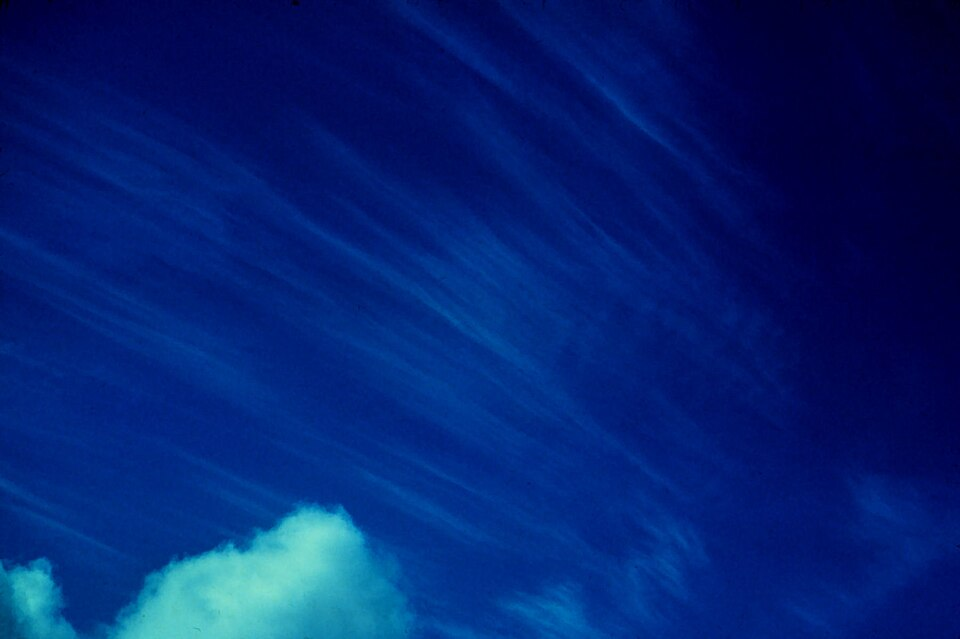
\includegraphics[width=\linewidth]{images/book1/g4-cirrus.jpg}

{\small \omterm{def:g4:clouds-rain-snow:cloud-families}{Sirus}: benang-benang es yang tipis, sangat tinggi (di bawahnya ada \omterm{def:g4:clouds-rain-snow:cloud-families}{kumulus} kecil).}
\end{minipage}\hfill
\begin{minipage}[b]{0.49\linewidth}\centering
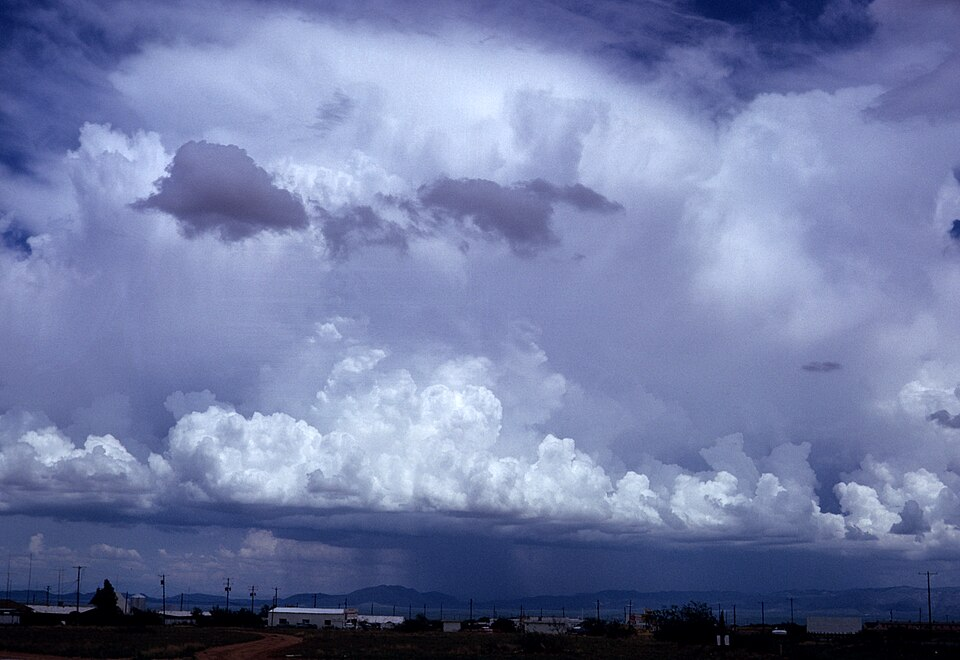
\includegraphics[width=\linewidth]{images/book1/g4-cumulonimbus.jpg}

{\small \omterm{def:g4:clouds-rain-snow:cloud-families}{Kumulonimbus}: menara \omterm{def:g4:clouds-rain-snow:cloud}{awan}; \omterm{def:g4:clouds-rain-snow:precipitation}{hujan} turun dari alasnya yang gelap.}
\end{minipage}

\smallskip
{\small Foto: NOAA Photo Library (domain publik): S. Corfidi (\omterm{def:g4:clouds-rain-snow:cloud-families}{kumulus}),
R. F. Kresge (\omterm{def:g4:clouds-rain-snow:cloud-families}{sirus}), koleksi B. Hooke (\omterm{def:g4:clouds-rain-snow:cloud-families}{kumulonimbus}).}
% ledger: noaa:photos-g4
\label{fig:g4:clouds-rain-snow:photos}
\end{omfigure}

Seberapa tinggi \omterm{def:g4:clouds-rain-snow:cloud}{awan} melayang? Itu bergantung pada golongannya. \omterm{def:g4:clouds-rain-snow:cloud}{Awan}
rendah, seperti \omterm{def:g4:clouds-rain-snow:cloud-families}{stratus} dan alas \omterm{def:g4:clouds-rain-snow:cloud-families}{kumulus}, melayang dari sedikit di atas
tanah sampai sekitar 2 kilometer. \omterm{def:g4:clouds-rain-snow:cloud-families}{Sirus} melayang sangat tinggi, antara
sekitar 5 dan 13 kilometer di luar daerah tropis dan daerah kutub --- sering
lebih tinggi daripada \omterm{def:g1:landscapes-around-us:landform}{gunung} tertinggi di Bumi.
\omterm{def:g4:clouds-rain-snow:cloud-families}{Kumulonimbus} membentang dari alas yang rendah sampai ke bagian paling atas
tingkat-tingkat \omterm{def:g4:clouds-rain-snow:cloud}{awan}.
% ledger: wmo:cloud-levels, wmo:cumulonimbus

\begin{omfigure}
\begin{tikzpicture}[x=1cm, y=0.5cm, font=\small]
  % height scale
  \draw[black!60] (0,0) -- (0,14);
  \foreach \h in {0,2,...,14} {
    \draw[black!60] (-0.1,\h) -- (0,\h);
    \node[anchor=east, font=\scriptsize] at (-0.12,\h) {\h\,km};
  }
  \node[anchor=south, font=\scriptsize, align=center] at (0,14.2) {ketinggian};
  % ground and a mountain for comparison
  \fill[green!35!black!50] (0.2,0) -- (11.4,0) -- (11.4,-0.4) -- (0.2,-0.4) -- cycle;
  \fill[black!35] (8.6,0) -- (9.9,8.8) -- (10.2,8.4) -- (11.2,0) -- cycle;
  \fill[white, draw=black!45, line width=0.3pt] (9.65,7.2) -- (9.9,8.8) -- (10.2,8.4) -- (10.4,7.0) -- (10.1,7.4) -- (9.9,7.0) -- cycle;
  \node[font=\scriptsize, align=center] at (9.9,10.2) {gunung\\tertinggi};
  % levels
  \fill[blue!6] (0.2,0.15) rectangle (8.3,2);
  \fill[blue!10] (0.2,5) rectangle (8.3,13);
  \node[anchor=west, font=\scriptsize, text=blue!50!black] at (0.3,1.65) {awan rendah};
  \node[anchor=west, font=\scriptsize, text=blue!50!black] at (0.3,12.6) {awan tinggi};
  % stratus: a flat grey layer
  \fill[black!25, rounded corners=2pt] (0.6,0.6) rectangle (2.6,1.3);
  \node[font=\scriptsize] at (1.6,-1.1) {stratus};
  % cumulus
  \pic[scale=0.7, transform shape] at (4.0,0.9) {puffycloud};
  \node[font=\scriptsize] at (4.0,-1.1) {kumulus};
  % cirrus: wisps
  \foreach \y in {9.4,10.0,10.6} {
    \draw[black!50, line width=0.6pt] (0.8,\y) .. controls (1.4,\y+0.5) and (2.0,\y+0.1) .. (2.6,\y+0.6);
  }
  \node[font=\scriptsize] at (1.7,8.5) {sirus};
  % cumulonimbus: tower with an anvil
  \fill[black!15, draw=black!45, line width=0.4pt]
    (5.4,1.0) .. controls (5.2,4) and (5.6,8) .. (5.9,11.2)
    .. controls (5.0,11.6) and (4.6,12.0) .. (4.8,12.3)
    -- (8.1,12.3) .. controls (8.2,12.0) and (7.8,11.6) .. (7.0,11.2)
    .. controls (7.3,8) and (7.6,4) .. (7.4,1.0) -- cycle;
  \fill[black!45] (5.4,1.0) rectangle (7.4,1.4);
  \foreach \x in {5.7,6.1,6.5,6.9,7.2}
    \draw[omWxRain, line width=0.6pt] (\x,0.95) -- (\x-0.15,0.15);
  \node[font=\scriptsize] at (6.4,-1.1) {kumulonimbus};
\end{tikzpicture}

{\small Ketinggian tempat keempat golongan \omterm{def:g4:clouds-rain-snow:cloud}{awan} melayang (ketinggian dalam
kilometer, untuk daerah yang bukan tropis dan bukan kutub). \omterm{def:g4:clouds-rain-snow:cloud-families}{Stratus} dan
alas \omterm{def:g4:clouds-rain-snow:cloud-families}{kumulus} rendah; \omterm{def:g4:clouds-rain-snow:cloud-families}{sirus} sering lebih tinggi daripada \omterm{def:g1:landscapes-around-us:landform}{gunung} tertinggi.
\omterm{def:g4:clouds-rain-snow:cloud-families}{Kumulonimbus} membentang dari alas yang rendah sampai ke puncak
tingkat-tingkat \omterm{def:g4:clouds-rain-snow:cloud}{awan}. Ketinggian menurut atlas \omterm{def:g4:clouds-rain-snow:cloud}{awan} Organisasi Meteorologi
Dunia.}
\label{fig:g4:clouds-rain-snow:heights}
% ledger: wmo:cloud-levels, tht:everest
\end{omfigure}

\begin{method}[Menamai awan]\label{met:g4:clouds-rain-snow:naming}
Lihatlah langit dan ajukan tiga pertanyaan:
\begin{enumerate}
  \item Apakah \omterm{def:g4:clouds-rain-snow:cloud}{awan} itu berupa tumpukan dengan alas yang datar? Kalau ya,
        itulah \omterm{def:g4:clouds-rain-snow:cloud-families}{kumulus} --- dan jika \omterm{def:g4:clouds-rain-snow:cloud}{awan} itu menjulang menjadi menara raksasa
        yang gelap, \omterm{def:g4:clouds-rain-snow:cloud-families}{kumulonimbus}.
  \item Apakah \omterm{def:g4:clouds-rain-snow:cloud}{awan} itu berupa lembaran yang datar dan rata yang
        menyembunyikan seluruh langit? Kalau ya, itulah \omterm{def:g4:clouds-rain-snow:cloud-families}{stratus}.
  \item Apakah \omterm{def:g4:clouds-rain-snow:cloud}{awan} itu tersusun dari benang-benang putih yang tipis, sangat
        tinggi? Kalau ya, itulah \omterm{def:g4:clouds-rain-snow:cloud-families}{sirus}.
\end{enumerate}
\end{method}

\begin{remark}[Awan memberi tahu cuaca]\label{rem:g4:clouds-rain-snow:tell}
\omterm{def:g4:clouds-rain-snow:cloud-families}{Kumulus} kecil di langit biru berarti \omterm{def:g1:watching-the-weather:weather}{cuaca} cerah. \omterm{def:g4:clouds-rain-snow:cloud-families}{Stratus} yang kelabu
membawa hari yang muram, kadang-kadang dengan gerimis. \omterm{def:g4:clouds-rain-snow:cloud-families}{Kumulonimbus} membawa
\omterm{def:g4:clouds-rain-snow:precipitation}{hujan} deras yang singkat, sering disertai guntur, kilat, dan embusan angin
kencang --- kadang-kadang \omterm{def:g4:clouds-rain-snow:precipitation}{hujan es}. \omterm{def:g4:clouds-rain-snow:cloud-families}{Sirus} tidak membawa \omterm{def:g4:clouds-rain-snow:precipitation}{hujan}, tetapi
ketika \omterm{def:g4:clouds-rain-snow:cloud-families}{sirus} menyebar dan menebal, \omterm{def:g4:clouds-rain-snow:precipitation}{hujan} sering turun sehari kemudian.
\end{remark}

\section{Hujan, salju, dan hujan es}

Di dalam \omterm{def:g4:clouds-rain-snow:cloud}{awan}, titik-titik air yang sangat kecil saling bertumbukan dan
bergabung, atau kristal-kristal es tumbuh dengan mengambil air dari
titik-titik air itu. Titik air \omterm{def:g4:clouds-rain-snow:cloud}{awan}, atau kristal es, yang sudah cukup
besar dan berat tidak bisa melayang lagi: ia jatuh.

\begin{definition}[Presipitasi]\label{def:g4:clouds-rain-snow:precipitation}
Yang disebut \emph{presipitasi}\index{presipitasi} adalah air yang jatuh
dari \omterm{def:g4:clouds-rain-snow:cloud}{awan} ke tanah: \emph{hujan}\index{hujan} (tetes-tetes air cair),
\emph{salju}\index{salju} (kepingan yang tersusun dari kristal-kristal es
yang saling melekat), atau \emph{hujan es}\index{hujan es} (butiran es yang
bulat, yang jatuh dari \omterm{def:g4:clouds-rain-snow:cloud}{awan} badai).
\end{definition}

Apakah yang turun \omterm{def:g4:clouds-rain-snow:precipitation}{hujan} atau \omterm{def:g4:clouds-rain-snow:precipitation}{salju} bergantung pada suhu udara yang dilalui
\omterm{def:g4:clouds-rain-snow:precipitation}{presipitasi} itu. Kepingan \omterm{def:g4:clouds-rain-snow:precipitation}{salju} terbentuk tinggi di dalam \omterm{def:g4:clouds-rain-snow:cloud}{awan} yang dingin.
Jika udara di bawahnya cukup lama bersuhu di atas \SI{0}{\celsius},
kepingan itu mencair dalam perjalanan turun dan sampai kepada kita sebagai
\omterm{def:g4:clouds-rain-snow:precipitation}{hujan}. Jika udara membeku sepanjang jalan sampai ke tanah, kepingan itu
tiba sebagai \omterm{def:g4:clouds-rain-snow:precipitation}{salju}.

\begin{omfigure}

\includegraphics[width=0.55\linewidth]{images/book1/ai/g4-snowflakes.jpg}

{\small Anak-anak menangkap kepingan \omterm{def:g4:clouds-rain-snow:precipitation}{salju} pada sarung tangan yang gelap:
setiap kepingan tersusun dari kristal-kristal es.}
\end{omfigure}

\omterm{def:g4:clouds-rain-snow:precipitation}{Hujan es} hanya turun dari \omterm{def:g4:clouds-rain-snow:cloud-families}{kumulonimbus}. Di dalam menara \omterm{def:g4:clouds-rain-snow:cloud}{awan} itu, angin
yang kuat ke atas membawa butiran es naik dan turun beberapa kali; setiap
perjalanan menambahkan lapisan es yang baru, seperti lapisan-lapisan
bawang, sampai butiran es itu terlalu berat untuk ditahan angin.

\begin{omfigure}
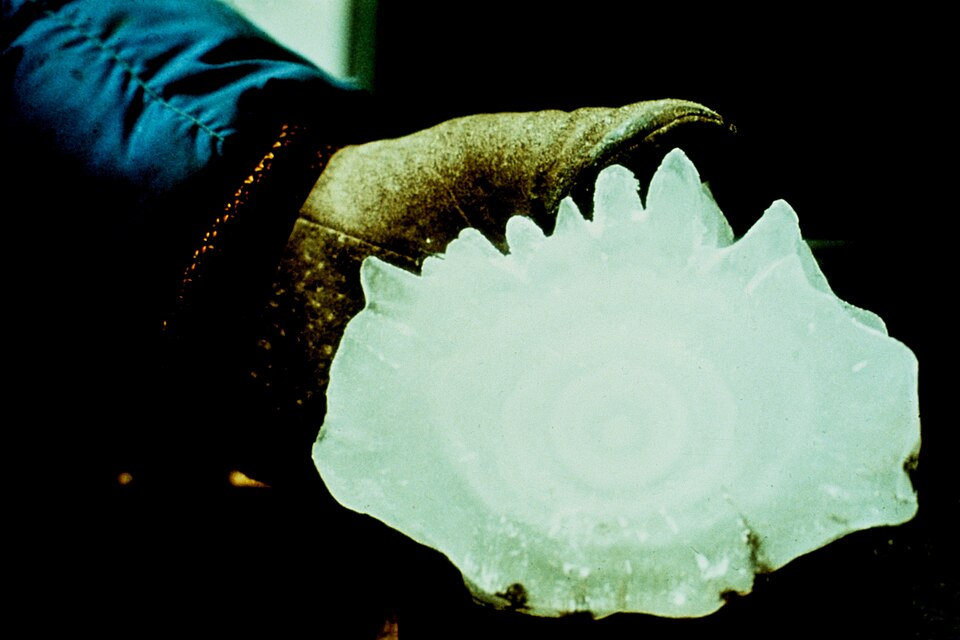
\includegraphics[width=0.5\linewidth]{images/book1/g4-hailstone.jpg}

{\small Butiran \omterm{def:g4:clouds-rain-snow:precipitation}{hujan es} yang sangat besar di tangan bersarung.
Cincin-cincinnya menunjukkan lapisan-lapisan es yang dikumpulkannya di
dalam \omterm{def:g4:clouds-rain-snow:cloud}{awan} badai. Foto: NOAA Photo Library (domain publik).}
% ledger: noaa:photos-g4
\end{omfigure}

\section{Mengukur cuaca}

Untuk menyatakan berapa banyak \omterm{def:g4:clouds-rain-snow:precipitation}{hujan} yang turun, seberapa hangat udara,
atau dari mana angin bertiup, kata-kata saja tidak cukup: kita memerlukan
alat ukur, dan angka.

\begin{definition}[Penakar hujan]\label{def:g4:clouds-rain-snow:rain-gauge}
Yang disebut \emph{penakar hujan}\index{penakar hujan} adalah wadah yang
menampung \omterm{def:g4:clouds-rain-snow:precipitation}{hujan} yang jatuh ke mulutnya. Kedalaman air yang ditampungnya
diukur dalam milimeter: ``\omterm{def:g4:clouds-rain-snow:precipitation}{hujan} 5 milimeter'' berarti \omterm{def:g4:clouds-rain-snow:precipitation}{hujan} itu akan
membentuk lapisan air setebal 5 milimeter di atas tanah yang datar,
seandainya tidak ada yang mengalir pergi atau meresap.
\end{definition}

\begin{remark}[Hujan satu milimeter itu banyak sekali airnya]\label{rem:g4:clouds-rain-snow:litre}
\omterm{def:g4:clouds-rain-snow:precipitation}{Hujan} satu milimeter tampak sangat sedikit di dalam penakar. Tetapi di atas
sepetak tanah berukuran satu meter kali satu meter, \omterm{def:g4:clouds-rain-snow:precipitation}{hujan} itu sama dengan
satu liter air: sebotol besar. Di halaman sekolah seluas seribu meter
persegi, \omterm{def:g4:clouds-rain-snow:precipitation}{hujan} 10 milimeter membawa sepuluh ribu liter: cukup untuk
mengisi seribu ember yang masing-masing berisi 10 liter.
\end{remark}

\begin{omfigure}
\begin{tikzpicture}[font=\small]
  % funnel
  \draw[black!70, line width=0.8pt] (-1.2,6.6) -- (-0.35,5.8) -- (-0.35,5.4);
  \draw[black!70, line width=0.8pt] (1.2,6.6) -- (0.35,5.8) -- (0.35,5.4);
  \draw[black!70, line width=0.8pt] (-1.2,6.6) -- (1.2,6.6);
  % tube
  \fill[blue!25] (-0.45,0) rectangle (0.45,2.4);
  \draw[black!70, line width=0.8pt] (-0.45,5.4) -- (-0.45,0) -- (0.45,0) -- (0.45,5.4);
  \foreach \m in {0,1,...,50} {
    \pgfmathsetmacro{\yy}{\m*0.1}
    \draw[black!60] (0.45,\yy) -- ++(-0.12,0);
  }
  \foreach \m in {0,5,10,...,50} {
    \pgfmathsetmacro{\yy}{\m*0.1}
    \draw[black!80] (0.45,\yy) -- ++(-0.25,0);
    \node[anchor=west, font=\scriptsize] at (0.5,\yy) {\m};
  }
  \node[anchor=west, font=\scriptsize] at (1.0,5.0) {mm};
  % reading line
  \draw[red!70!black, -{Stealth}] (-1.6,2.4) -- (-0.5,2.4);
  \node[anchor=east, align=right, font=\scriptsize] at (-1.65,2.4) {bacalah\\permukaannya di sini};
  \node[anchor=west, font=\scriptsize] at (1.9,2.4) {$\leftarrow$ hujan 24\,mm};
\end{tikzpicture}

{\small \omterm{def:g4:clouds-rain-snow:rain-gauge}{Penakar hujan} sederhana: corong menangkap \omterm{def:g4:clouds-rain-snow:precipitation}{hujan}, dan tabung yang
diberi tanda milimeter menampungnya. Bacalah permukaan airnya, dengan
matamu sejajar dengannya. Di sini, 24 milimeter \omterm{def:g4:clouds-rain-snow:precipitation}{hujan} sudah turun sejak
penakar itu terakhir dikosongkan.}
\label{fig:g4:clouds-rain-snow:gauge}
\end{omfigure}


\begin{definition}[Penunjuk arah angin]\label{def:g4:clouds-rain-snow:wind-vane}
Yang disebut \emph{penunjuk arah angin}\index{penunjuk arah angin} adalah
anak panah yang berputar bebas pada sebuah tiang. Angin mendorong ekornya,
sehingga anak panah itu selalu menunjuk ke arah \emph{asal} angin.
\end{definition}

\begin{definition}[Stasiun cuaca]\label{def:g4:clouds-rain-snow:weather-station}
Yang disebut \emph{stasiun cuaca}\index{stasiun cuaca} adalah tempat \omterm{def:g1:watching-the-weather:weather}{cuaca}
diukur setiap hari, selalu dengan cara yang sama, memakai alat-alat ukur:
termometer di dalam kotak putih yang berventilasi, \omterm{def:g4:clouds-rain-snow:rain-gauge}{penakar hujan} di tempat
terbuka, dan \omterm{def:g4:clouds-rain-snow:wind-vane}{penunjuk arah angin} di atas tiang.
\end{definition}

Termometer diletakkan di tempat teduh, di dalam kotak putih yang dindingnya
berkisi-kisi, yang membiarkan udara masuk tetapi menahan sinar matahari dan
\omterm{def:g4:clouds-rain-snow:precipitation}{hujan}. Met Office, dinas \omterm{def:g1:watching-the-weather:weather}{cuaca} Britania Raya, memasangnya
\SI{1.25}{\metre} di atas tanah. \omterm{def:g4:clouds-rain-snow:rain-gauge}{Penakar hujan}
berdiri di tempat terbuka, jauh dari dinding dan pohon yang akan
menghalanginya dari \omterm{def:g4:clouds-rain-snow:precipitation}{hujan}, dengan mulutnya sedikit di atas tanah.
\omterm{def:g4:clouds-rain-snow:wind-vane}{Penunjuk arah angin} berdiri tinggi di atas tiangnya, di atas
penghalang-penghalang yang akan membelokkan angin.
% ledger: mo:screen-height, mo:raingauge

\begin{omfigure}
\begin{tikzpicture}[font=\small, x=1cm, y=1cm]
  % grass
  \fill[green!40!black!45] (-0.5,0) rectangle (11,-0.25);
  \foreach \x in {-0.3,0.1,...,10.8} \draw[green!45!black] (\x,0) -- ++(0.06,0.14);
  % screen on legs
  \draw[black!70, line width=1pt] (0.8,0) -- (0.8,1.25) (2.2,0) -- (2.2,1.25);
  \fill[white, draw=black!70] (0.6,1.25) rectangle (2.4,2.4);
  \foreach \y in {1.4,1.55,...,2.25} \draw[black!40] (0.7,\y) -- (2.3,\y-0.08);
  \fill[white, draw=black!70] (0.45,2.4) -- (1.5,2.75) -- (2.55,2.4) -- cycle;
  \draw[black!60, <->] (2.8,0) -- node[right, font=\scriptsize, align=left] {sekitar\\1.25\,m} (2.8,1.25);
  \node[align=center, font=\scriptsize] at (1.5,3.25) {termometer di dalam\\kotak putih berkisi-kisi};
  % rain gauge
  \fill[black!15, draw=black!70] (5.4,0) rectangle (5.9,0.4);
  \draw[black!70] (5.3,0.55) -- (5.4,0.4) (6.0,0.55) -- (5.9,0.4);
  \node[align=center, font=\scriptsize] at (5.65,1.2) {penakar hujan,\\di tempat terbuka};
  % tree far away
  \fill[brown!60!black] (7.3,0) rectangle (7.5,1.3);
  \fill[green!50!black!70] (7.4,2.1) circle (0.85);
  % wind vane on a mast
  \draw[black!70, line width=1pt] (9.8,0) -- (9.8,4.2);
  \draw[black!80, line width=1.4pt, -{Latex[length=3mm]}] (10.6,4.4) -- (9.0,4.4);
  \fill[black!80] (10.6,4.4) -- (10.9,4.65) -- (10.9,4.15) -- cycle;
  \node[align=center, font=\scriptsize] at (9.8,5.05) {penunjuk arah angin di atas tiang tinggi};
  \node[anchor=west, font=\scriptsize, align=left] at (10.1,3.4) {menunjuk ke\\asal angin};
\end{tikzpicture}

{\small Sebuah \omterm{def:g4:clouds-rain-snow:weather-station}{stasiun cuaca} kecil. Termometer ada di tempat teduh, di dalam
kotak putih yang dindingnya berkisi-kisi, sekitar 1.25 meter di atas
rumput; \omterm{def:g4:clouds-rain-snow:rain-gauge}{penakar hujan} berdiri di tempat terbuka, jauh dari pohon; \omterm{def:g4:clouds-rain-snow:wind-vane}{penunjuk
arah angin} berada tinggi di atas penghalang.}
\label{fig:g4:clouds-rain-snow:station}
% ledger: mo:screen-height
\end{omfigure}

\begin{inthefield}[Stasiun cuaca di halaman sekolah]
Banyak sekolah memiliki \omterm{def:g4:clouds-rain-snow:weather-station}{stasiun cuaca} kecil di sudut halaman bermain.
Setiap pagi pada jam yang sama, dua murid membaca termometer, membaca dan
mengosongkan \omterm{def:g4:clouds-rain-snow:rain-gauge}{penakar hujan}, dan mencatat ke mana \omterm{def:g4:clouds-rain-snow:wind-vane}{penunjuk arah angin}
menunjuk. Dari minggu ke minggu, kelas itu menyusun catatan \omterm{def:g1:watching-the-weather:weather}{cuacanya}
sendiri.
\end{inthefield}

\begin{omfigure}
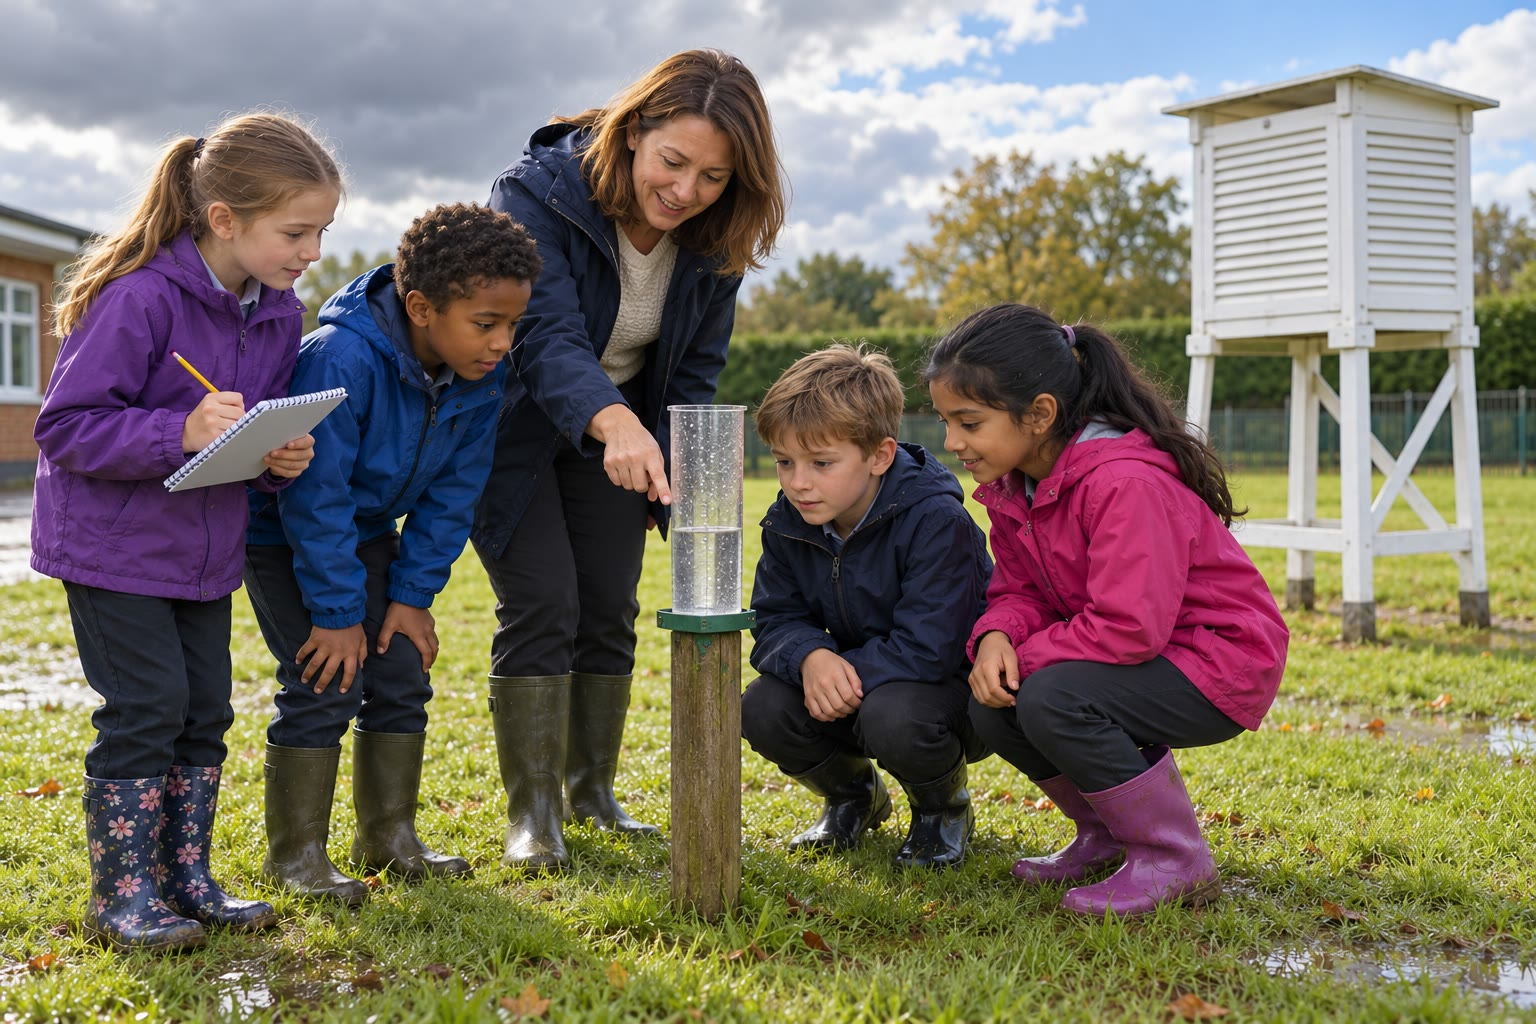
\includegraphics[width=0.55\linewidth]{images/book1/ai/g4-rain-gauge-class.jpg}

{\small Murid-murid membaca \omterm{def:g4:clouds-rain-snow:rain-gauge}{penakar hujan} di halaman sekolah.}
\end{omfigure}

\begin{method}[Menggambar diagram batang curah hujan]\label{met:g4:clouds-rain-snow:bar-chart}
Untuk menggambar curah \omterm{def:g4:clouds-rain-snow:precipitation}{hujan} selama seminggu:
\begin{enumerate}
  \item gambarlah garis mendatar dan tuliskan hari-hari di bawahnya, dengan
        jarak yang sama;
  \item gambarlah garis tegak di sebelah kiri dan beri tanda dalam
        milimeter, dengan langkah yang sama (misalnya setiap 2 milimeter);
  \item di atas setiap hari, gambarlah sebuah batang setinggi curah \omterm{def:g4:clouds-rain-snow:precipitation}{hujan}
        hari itu; hari tanpa \omterm{def:g4:clouds-rain-snow:precipitation}{hujan} tidak mendapat batang sama sekali;
  \item berilah diagram itu judul dan tuliskan satuannya, mm, pada garis
        tegak.
\end{enumerate}
\end{method}

\begin{example}[Seminggu hujan di sekolah]\label{ex:g4:clouds-rain-snow:week}
Kelas itu membaca \omterm{def:g4:clouds-rain-snow:rain-gauge}{penakar hujan} setiap pagi selama seminggu dan
mendapatkan: Senin 0, Selasa 4, Rabu 12, Kamis 7, Jumat 0, Sabtu 2, Minggu
5 milimeter. Hari yang paling basah adalah Rabu. Tidak turun \omterm{def:g4:clouds-rain-snow:precipitation}{hujan} pada
hari Senin maupun Jumat. Selama seminggu penuh, turun
$0 + 4 + 12 + 7 + 0 + 2 + 5 = 30$ milimeter. Hari Rabu saja membawa 12 dari
30 milimeter itu, yaitu $\frac{12}{30} = \frac{2}{5}$ dari curah \omterm{def:g4:clouds-rain-snow:precipitation}{hujan}
minggu itu.
\end{example}

\begin{omfigure}
\begin{tikzpicture}
\begin{axis}[ybar, bar width=14pt, width=0.8\linewidth, height=5.4cm,
    ymin=0, ymax=14, ytick={0,2,...,14}, ylabel={hujan (mm)},
    symbolic x coords={Mon,Tue,Wed,Thu,Fri,Sat,Sun}, xtick=data, xticklabels={Sen,Sel,Rab,Kam,Jum,Sab,Min},
    axis x line*=bottom, axis y line*=left, ymajorgrids, grid style={gray!25},
    nodes near coords, nodes near coords style={font=\scriptsize},
    every axis label/.append style={font=\small}, tick label style={font=\small},
    title={Hujan di sekolah, satu minggu}, title style={font=\small}]
  \addplot[fill=omWxRain!70, draw=omWxRain!60!black] coordinates
    {(Mon,0) (Tue,4) (Wed,12) (Thu,7) (Fri,0) (Sat,2) (Sun,5)};
\end{axis}
\end{tikzpicture}

{\small Minggu pada \cref{ex:g4:clouds-rain-snow:week} dalam bentuk diagram batang.}
\label{fig:g4:clouds-rain-snow:bars}
\end{omfigure}

\section{Latihan}

\begin{exercise}[$\star$]\label{exo:g4:clouds-rain-snow:1}
Terbuat dari apakah \omterm{def:g4:clouds-rain-snow:cloud}{awan}? Apa itu \omterm{def:g4:clouds-rain-snow:cloud}{kabut}?
\end{exercise}

\begin{exercise}[$\star$]\label{exo:g4:clouds-rain-snow:2}
Sebutkan nama \omterm{def:g4:clouds-rain-snow:cloud}{awannya}: (a) lembaran kelabu yang datar yang menyembunyikan
seluruh langit; (b) benang-benang putih yang tipis, sangat tinggi di langit
biru; (c) tumpukan putih dengan alas datar, seperti kapas; (d) menara
raksasa yang gelap dengan puncak datar, yang membawa guntur.
\end{exercise}

\begin{exercise}[$\star$]\label{exo:g4:clouds-rain-snow:3}
\omterm{def:g4:clouds-rain-snow:precipitation}{Hujan}, \omterm{def:g4:clouds-rain-snow:precipitation}{salju}, atau \omterm{def:g4:clouds-rain-snow:precipitation}{hujan es}? (a) butiran es bulat yang jatuh dari \omterm{def:g4:clouds-rain-snow:cloud}{awan}
badai; (b) tetes-tetes air cair; (c) kepingan yang tersusun dari
kristal-kristal es.
\end{exercise}

\begin{exercise}[$\star$]\label{exo:g4:clouds-rain-snow:4}
Alat apa yang mengukur: (a) \omterm{def:g4:clouds-rain-snow:precipitation}{hujan}; (b) suhu; (c) arah asal angin?
\end{exercise}

\begin{exercise}[$\star$]\label{exo:g4:clouds-rain-snow:5}
Pada \omterm{def:g4:clouds-rain-snow:rain-gauge}{penakar hujan} yang digambar di halaman~\pageref{fig:g4:clouds-rain-snow:gauge},
air sekarang mencapai tanda 17. Berapa milimeter \omterm{def:g4:clouds-rain-snow:precipitation}{hujan} yang sudah turun?
Berapa milimeter lagi yang diperlukan untuk mencapai 20?
\end{exercise}

\begin{exercise}[$\star$]\label{exo:g4:clouds-rain-snow:6}
Lihatlah diagram batang di halaman~\pageref{fig:g4:clouds-rain-snow:bars}.
Hari apa yang paling basah? Pada hari apa saja tidak turun \omterm{def:g4:clouds-rain-snow:precipitation}{hujan}? Hari apa
yang mendapat 7 milimeter?
\end{exercise}

\begin{exercise}[$\star\star$]\label{exo:g4:clouds-rain-snow:7}
Pada pagi hari yang bersalju, kepingan \omterm{def:g4:clouds-rain-snow:precipitation}{salju} sampai ke tanah di desa
pegunungan, tetapi di \omterm{def:g1:landscapes-around-us:landform}{lembah} di bawahnya turun \omterm{def:g4:clouds-rain-snow:precipitation}{hujan}. Jelaskan perbedaan
itu dengan memakai suhu udara.
\end{exercise}

\begin{exercise}[$\star\star$]\label{exo:g4:clouds-rain-snow:8}
Pada minggu yang lain, kelas itu mendapatkan: Senin 3, Selasa 0, Rabu 1,
Kamis 9, Jumat 6, Sabtu 0, Minggu 1 milimeter. Gambarlah diagram
batangnya. Berapa milimeter yang turun dalam minggu itu? Berapa bagian
dari curah \omterm{def:g4:clouds-rain-snow:precipitation}{hujan} minggu itu yang turun pada hari Kamis?
\end{exercise}

\begin{exercise}[$\star\star$]\label{exo:g4:clouds-rain-snow:9}
Mengapa \omterm{def:g4:clouds-rain-snow:rain-gauge}{penakar hujan} harus berdiri di tempat terbuka, jauh dari dinding
dan pohon? Mengapa termometer disimpan di dalam kotak putih di tempat
teduh, dan tidak di bawah terik matahari?
\end{exercise}

\begin{exercise}[$\star\star$]\label{exo:g4:clouds-rain-snow:10}
\omterm{def:g4:clouds-rain-snow:wind-vane}{Penunjuk arah angin} menunjuk ke barat. Dari mana angin datang? Ke mana
angin pergi?
\end{exercise}

\begin{exercise}[$\star\star\star$]\label{exo:g4:clouds-rain-snow:11}
Di halaman bermain seluas 500 meter persegi turun \omterm{def:g4:clouds-rain-snow:precipitation}{hujan} 8 milimeter.
Dengan memakai \cref{rem:g4:clouds-rain-snow:litre}, berapa liter air yang
jatuh di halaman bermain itu? Sebuah gembor berisi 10 liter: berapa gembor
banyaknya air itu?
\end{exercise}
